\documentclass[t,12pt,aspectratio=169]{beamer}
% ==========================================================
% 1. PENGATURAN BAHASA & ENCODING
% ==========================================================
\usepackage[bahasa]{babel}      % Penyesuaian format tanggal/nama Indonesia
\usepackage[utf8]{inputenc}     % Encoding karakter standar
\usepackage[T1]{fontenc}        % Encoding font output
\usepackage{physics}

\usepackage{booktabs}
\usepackage[table]{xcolor}
\usepackage{graphicx}

% ==========================================================
% 2. PENGATURAN FONT (Comic Style + Math Euler)
% ==========================================================
% --- Font Teks ---
\usepackage[scaled=1.2]{comicneue}  
\renewcommand{\familydefault}{\sfdefault}
\usefonttheme{structurebold}

% --- Font Matematika ---
\usefonttheme[onlymath]{serif}     % Matematika serif
\usepackage{mathpazo}              % Palatino untuk operator
\usepackage{eulervm}               % Euler untuk variabel 

% FIX: Sembunyikan warning bahwa hbar diganti hslash
\usepackage{silence}
\WarningFilter{eulervm}{Symbol \hbar not available}
\usepackage{eulervm}

% --- TEKNIK PENEBALAN TEKS (MICRO-STROKE) ---
% Menambahkan garis tepi tipis agar font terlihat lebih tebal
% Sesuaikan LineWidth: 0.1pt (Tipis) s.d 0.4pt (Tebal)
\usepackage{pdfrender}
\AtBeginDocument{
    \pdfrender{
        TextRenderingMode=FillStroke,
        LineWidth=0.2pt,  % <--- Ubah untuk atur ketebalan
        FillColor=.,      % Warna isi mengikuti teks saat ini
        StrokeColor=.     % Warna garis tepi mengikuti teks saat ini
    }
}

% --- Pengaturan Vektor (Gaya Papan Tulis) ---
%\usepackage[d]{esvect}             
%\renewcommand{\vec}{\vv}
\usepackage{bbm} 
\renewcommand{\mathbf}[1]{\mathbbm{#1}}

% ==========================================================
% 3. PAKET MATEMATIKA & ALGORITMA
% ==========================================================
\usepackage{amsmath,amssymb}
\usepackage{algorithm}         
\usepackage{algpseudocode}

% ==========================================================
% 4. PENGATURAN SPASI & LAYOUT TEKS
% ==========================================================
\usepackage{xpatch}             

% Mengatur jarak antar paragraf
\setlength{\parskip}{0.5em}

% Patch untuk memberi jarak antar item list (bullet points)
% Itemize (Bullet) -> 0.4em
\xpatchcmd{\itemize}{\def\makelabel}{\setlength{\itemsep}{0.4em}\def\makelabel}{}{}
% Enumerate (Angka) -> 0.6em
\xpatchcmd{\enumerate}{\def\makelabel}{\setlength{\itemsep}{0.6em}\def\makelabel}{}{}

% Margin Kiri/Kanan Slide
\setbeamersize{text margin left=1cm, text margin right=1cm}

% ==========================================================
% 5. GRAFIK, WARNA & TIKZ
% ==========================================================
\usepackage{graphicx}
\usepackage{pdfpages} 
\usepackage{tikz, pgfplots}
\usetikzlibrary{shapes, arrows.meta, positioning, calc, backgrounds, fit, shadows, decorations.pathmorphing}
\pgfplotsset{compat=1.18}
\tikzset{wave/.style={decorate, decoration={snake, amplitude=2pt, segment length=8pt}}}

% --- Definisi Palet Warna (Chalk/Kapur) ---
\definecolor{cb}{RGB}{85, 160, 220}   % Chalk Blue
\definecolor{cr}{RGB}{219, 112, 147}  % Chalk Red 
\definecolor{co}{RGB}{255, 170, 80}   % Chalk Orange
\definecolor{cg}{RGB}{140, 220, 140}  % Chalk Green 
\definecolor{cw}{RGB}{240, 240, 240}  % Chalk White 
\definecolor{BoardDeep}{HTML}{111111} % Background Gelap

% --- FIX TIKZ PICTURE (TOTAL RESET) ---
% Perintah ini akan mematikan efek "Fake Bold" khusus TikZ

\tikzset{
    every picture/.append style={
        execute at begin picture={
            % Reset mode ke "Fill" saja (tanpa garis tepi)
            \pdfrender{TextRenderingMode=Fill, LineWidth=0pt}
        }
    }
}

% ==========================================================
% 6. PENGATURAN KODE PROGRAM (MINTED)
% ==========================================================
\usepackage{minted}
\usemintedstyle{monokai}

\setminted[python]{
    fontsize=\footnotesize,   
    linenos=false,          
    breaklines=true,        
    tabsize=4,
    frame=none,             
    bgcolor={},             % Transparan (menyatu bg slide)
}

% ==========================================================
% 7. TEMA BEAMER: WARNA ELEMEN
% ==========================================================
% --- Warna Latar & Teks Utama ---
%\setbeamercolor{background canvas}{bg=BoardDeep} 

% Menggunakan file 'chalkboard.jpg' sebagai latar belakang
\usebackgroundtemplate{%
\tikz[overlay,remember picture] \node[opacity=1, at=(current page.center)] {
   % Pastikan file chalkboard.jpg ada di folder yang sama!
   \includegraphics[height=\paperheight, 
   width=\paperwidth]{templates/chalkboard.jpg}};
}
\setbeamercolor{normal text}{fg=cw}      

% --- Warna Header & Footer ---
\setbeamercolor{frametitle}{fg=white}
\setbeamercolor{title}{fg=cw}
\setbeamercolor{subtitle}{fg=cb}
\setbeamercolor{author}{fg=white!70!blue}
\setbeamercolor{institute}{fg=white!70!gray}
\setbeamercolor{date}{fg=white!70!gray}

% --- Warna Blok & Caption ---
\setbeamertemplate{blocks}[rounded][shadow=false]
\setbeamercolor{block title}{fg=cg, bg=black!85}
\setbeamercolor{block body}{fg=white, bg=black!80}
\setbeamercolor{block title alerted}{fg=cr, bg=black!60}
\setbeamercolor{block body alerted}{fg=cw, bg=black!30}
\setbeamercolor{block title example}{fg=co, bg=black!60}
\setbeamercolor{block body example}{fg=cw, bg=black!30}

% --- Caption ---
\setbeamercolor{caption}{fg=cg}

% --- Warna List (Itemize/Enumerate) ---
\setbeamertemplate{itemize items}{\color{co}$\blacktriangleright$} % Bullet Segitiga Oranye
\setbeamercolor{enumerate item}{fg=cb}        % Angka Biru
\setbeamercolor{enumerate subitem}{fg=cb}
\setbeamercolor{enumerate subsubitem}{fg=cb}

% ==========================================================
% 8. TEMA BEAMER: DAFTAR ISI (TOC)
% ==========================================================
% Menggunakan warna ungu manual (purple) untuk panah di TOC
\setbeamercolor{section in toc}{fg=cw}
\setbeamercolor{subsection in toc}{fg=cb}
\setbeamercolor{subsubsection in toc}{fg=white!50!gray}
\setbeamercolor{section number projected}{bg=blue!80, fg=black}
\setbeamercolor{toc title}{fg=yellow!80!white}

\setbeamertemplate{section in toc}{%
  \leavevmode
  \textcolor{cr}{$\bullet$}\hspace{1em}%
  \inserttocsection\par}

\setbeamertemplate{subsection in toc}{%
  \hspace{1.5em}%
  \textcolor{purple}{$\blacktriangleright$}\hspace{1em}%
  \inserttocsubsection\par}

% ==========================================================
% 9. TEMA BEAMER: TEMPLATE HEADER & TITLE
% ==========================================================
% Hilangkan simbol navigasi kecil
\setbeamertemplate{navigation symbols}{} 

% Format Judul Frame (Header)
\setbeamertemplate{frametitle}{
  \nointerlineskip
  \begin{beamercolorbox}[
    wd=\paperwidth,    
    sep=1cm,           
    leftskip=0cm,      
    rightskip=0.5cm    
  ]{frametitle}
    \usebeamerfont{frametitle}\insertframetitle
  \end{beamercolorbox}
  \vspace*{-1.5em} 
}

% Format Caption Gambar
\setbeamertemplate{caption}{
  \footnotesize
  {\usebeamercolor[fg]{caption}\insertcaption}\par
}

% Format Halaman Judul (Title Page)
\defbeamertemplate*{title page}{centered logo}{
  \begin{center}
    \vspace*{0.15\paperheight} % Slightly adjusted top margin  
    % Title
    {\usebeamerfont{title}\inserttitle\par}    
    % Subtitle
    \vspace{0.8ex}
    {\usebeamerfont{subtitle}\insertsubtitle\par}    
    % Author (Added)
    \vspace{1em}
    {\usebeamerfont{author}\insertauthor\par}
    % Institute (Added)
    \vspace{0.5em}{\usebeamerfont{institute}\footnotesize\insertinstitute\par}    
    \vfill    
    % Logo/Graphic
    {\usebeamerfont{institute}\inserttitlegraphic\par}
    \vspace*{-2em}
  \end{center}
}

\setbeamertemplate{title page}[centered logo]
% ==========================================================
% 10. CUSTOM COMMANDS (MACRO)
% ==========================================================
% Macro untuk menyisipkan gambar dengan bayangan
\newcommand{\shadowfig}[3][]{%
  \tikz\node[inner sep=0pt, drop shadow, #1]{\includegraphics[#2]{#3}};%
}

% Shortcut untuk transisi fade
\newcommand{\fade}{\transfade}

% Symbol for enter:
\newcommand{\enterRight}{\reflectbox{\ensuremath{\hookleftarrow}}\,}
%-----------------------------------------------------------
\title{\Large \textbf{Variational quantum (and classical) algorithms for Hamiltonian Simulation}}
\subtitle{QuaComputeID Meeting 2026.02.03}
\author{\textcolor{cr}{M. E. Ong} / \textcolor{cr}{Meng E. Ong} (@fisikawan.gendeng)\\
assisted by \textcolor{cr}{M. S. Fittuqo} (sophomore IT student from UGM)\\
\textcolor{cb}{https://github.com/Syauqi-dotcom/BRIN-Internship-2026}}
\titlegraphic{
% sesuaikan logo di bawah ini:
\includegraphics[width=1cm]{templates/quacompute.png}
}
%-----------------------------------------------------------
\begin{document}
%-----------------------------------------------------------
\begin{frame}
  \titlepage
\end{frame}
%-----------------------------------------------------------
\begin{frame}{Tonight's Menu}
%-----------------------------------------------------------
%    \begin{columns}[t]
%        \begin{column}{0.9\textwidth}
            \tableofcontents
%        \end{column}
%    \end{columns}
\end{frame}


%===========================================================
\section{Hamiltonian Simulation}
%===========================================================

%-----------------------------------------------------------
\begin{frame}{Hamiltonian simulation: electronic structure}
%-----------------------------------------------------------
\textbf{Molecular Orbital}

    Direct example: To calculate the hydrogen molecule ($H_2$) orbital, we employ the \textbf{LCAO (Linear Combination of Atomic Orbitals)} approximation.
    
    figsWe define the molecular wavefunction $\ket{\psi_{H_2}}$ as:
    \begin{align*}
        \ket{\psi_{H_2}} &= c_1 \ket{H_{1s}^{(1)}} + c_2 \ket{H_{1s}^{(2)}} \\ \\
        \ket{\psi} &= c_1 \ket{\phi_1} + c_2 \ket{\phi_2}
    \end{align*}

    \begin{center}
    \begin{tikzpicture}[scale=0.8]
        \draw[thick] (0, 2) -- (1.5, 2) node[left, at start] {$H_{1s}^{(1)}$ (Atom 1)};
        \draw[decorate, decoration={snake, amplitude=2pt, segment length=10pt}, gray!80] (1.5, 2) -- (4.5, 2);
        \draw[thick] (4.5, 2) -- (6, 2) node[right, at end] {(Atom 2) $H_{1s}^{(2)}$};
    \end{tikzpicture}
    \end{center}
\end{frame}

%-----------------------------------------------------------
\begin{frame}{How to Calculate Electronic Structure}
%-----------------------------------------------------------
    
\textbf{Solve Time-Independent Schrödinger Equation (TISE)}
    
  \vspace{0.5em}
    We substitute our LCAO ansatz into the time-independent Schrödinger Equation:
    \[
        \hat{H} \ket{\Psi} = E \ket{\Psi}
    \]

    We project the equation onto the basis state:
    \begin{align}
        \mel{\phi_i}{\hat{H}}{\Psi} &= E \braket{\phi_i}{\Psi} \label{eq:intro} \\
        \intertext{This step transforms the operator equation into a system of linear equations:}
        c_1 \mel{\phi_1}{\hat{H}}{\phi_1} + c_2 \mel{\phi_1}{\hat{H}}{\phi_2} &= E \left( c_1 \braket{\phi_1}{\phi_1} + c_2 \braket{\phi_1}{\phi_2} \right) \label{eq:1} \\
        c_1 \mel{\phi_2}{\hat{H}}{\phi_1} + c_2 \mel{\phi_2}{\hat{H}}{\phi_2} &= E \left( c_1 \braket{\phi_2}{\phi_1} + c_2 \braket{\phi_2}{\phi_2} \right) \label{eq:2}
    \end{align}
\end{frame}

%-----------------------------------------------------------
\begin{frame}{Characteristic Equation}
%-----------------------------------------------------------
    \textbf{Matrix Representation}

    $$
    \begin{bmatrix}
    H_{11} & H_{12} \\ 
    H_{21} & H_{22} 
    \end{bmatrix} 
    \begin{bmatrix} 
    c_1 \\ c_2 
    \end{bmatrix} = E 
    \begin{bmatrix} 
    S_{11} & S_{12} \\ 
    S_{21} & S_{22} 
    \end{bmatrix} 
    \begin{bmatrix} 
    c_1 \\ c_2 
    \end{bmatrix}
    $$
    $$
    \begin{bmatrix}
    \varepsilon & t \\ 
    t & \varepsilon 
    \end{bmatrix} 
    \begin{bmatrix} 
    c_1 \\ c_2 
    \end{bmatrix} = E 
    \begin{bmatrix} 
    1 & 0 \\ 
    0 & 1 
    \end{bmatrix} 
    \begin{bmatrix} 
    c_1 \\ c_2 
    \end{bmatrix}
    $$
       
    \vspace{0.em} 
    \small 
    \begin{itemize}
        \item $H_{ii} = \langle \phi_i | \hat{H} | \phi_i \rangle = \varepsilon$: \textbf{On-site Energy of an isolated atom} .
        \item $H_{ij} = \langle \phi_i | \hat{H} | \phi_j \rangle = t$: \textbf{Hopping Energy} (Transfer Integral)
        \item $S_{ij} = \langle \phi_i | \phi_j \rangle$: \textbf{Overlap Integral}, Assumed orthogonality for simplification ($S_{i,j} \approx 0, S_{i,i} \approx 1$).
    \end{itemize}
\end{frame}

%-----------------------------------------------------------
\begin{frame}{Characteristic Equation}
%-----------------------------------------------------------
    For the system of linear equations to have a non-trivial solution (where coefficients $c_1, c_2 \neq 0$), the determinant of the coefficient matrix must vanish:
    $$ \det(\mathbf{H} - E\mathbf{S}) = 0 $$
    Substituting our Tight-Binding parameters ($\varepsilon$ and $t$) and assuming orthogonality ($S \approx I$):
    $$\begin{vmatrix} \varepsilon - E & t \\ t & \varepsilon - E \end{vmatrix} = 0$$
    This yields two possible Energy Eigenvalues:
    $$ \boxed{E = \varepsilon \pm t} $$
\end{frame}

%-----------------------------------------------------------
\begin{frame}{Molecular Energy Levels}
%-----------------------------------------------------------
    \begin{columns}
        % Kolom Kiri: Penjelasan Teks
        \begin{column}{0.55 \textwidth}
            \textbf{Eigenvalue Solutions\\
            Note that $t < 0$ is assumed)}
            
            \vspace{1em}
            \structure{\textbf{\textcolor{cr}{Anti-Bonding State $(E_{-})$}}}
            $$E_{-} = \varepsilon - t \approx -11.6eV$$
        
            This state has a higher energy (\textcolor{cr}{unstable}) 
            
            \vspace{0.5em}
            \structure{\textbf{\textcolor{cg}{Bonding State($(E_+)$}}}
            $$ E_+ = \varepsilon + t \approx -15.6eV$$
        
            This state has a lower energy (\textcolor{cg}{stable})

        \end{column} 
        % Kolom Kanan: Diagram Energi
        \begin{column}{0.45\textwidth}
            \begin{center}
            \begin{tikzpicture}[scale=0.7]
                % Sumbu Energi
                \draw[->, thick] (-0.5, 0) -- (-0.5, 5) node[above] {Energy};

                % Level Atom (Kiri & Kanan) - Epsilon
                \draw[thick, cyan] (0, 2.5) -- (1.5, 2.5) node[midway, above] {$\varepsilon$};
                \draw[thick, cyan] (4.5, 2.5) -- (6, 2.5) node[midway, above] {$\varepsilon$};
                
                % Level Molekul (Tengah)
                % Anti-Bonding (E - t) -> Anggap t negatif, jadi ini E - t (lebih tinggi)
                \draw[thick, magenta] (2.25, 4.0) -- (3.75, 4.0) node[midway, above] {$E_- = \varepsilon - t$};
                \node[right, magenta, font=\tiny] at (3.75, 4.0) {($\sigma^*$ Anti-bonding)};
                
                % Bonding (E + t) -> Anggap t negatif, jadi ini E + t (lebih rendah)
                \draw[thick, green!60!black] (2.25, 1.0) -- (3.75, 1.0) node[midway, below] {$E_+ = \varepsilon + t$};
                \node[right, green!60!black, font=\tiny] at (3.75, 1.0) {($\sigma$ Bonding)};

                % Garis Putus-putus (Konektor)
                \draw[dashed, gray] (1.5, 2.5) -- (2.25, 4.0);
                \draw[dashed, gray] (1.5, 2.5) -- (2.25, 1.0);
                \draw[dashed, gray] (4.5, 2.5) -- (3.75, 4.0);
                \draw[dashed, gray] (4.5, 2.5) -- (3.75, 1.0);
                
            \end{tikzpicture}
            \end{center}
        \end{column}
    \end{columns}   
\end{frame}

%-----------------------------------------------------------
\begin{frame}{Electronic structure of hydrogen molecule}
%-----------------------------------------------------------
\textbf{Molecular Orbital Diagram $(H_2)$}
\vspace{0.5em}
\begin{columns}[T] 
        % --- KOLOM KIRI: DIAGRAM KOSONG ---
        \begin{column}{0.5\textwidth}
            \centering
            \begin{tikzpicture}[scale=0.7, every node/.style={transform shape}]
                % Sumbu Energi (Tulisan digeser ke samping dengan 'left=0.5cm')
                \draw[-{Latex}, thick] (0,0) -- (0,6) node[midway, left=0.5cm, rotate=90] {Energy};
                
                % Definisi Koordinat
                \coordinate (L_Atom) at (1, 3);      
                \coordinate (R_Atom) at (5, 3);      
                \coordinate (MO_Bonding) at (3, 1);   
                \coordinate (MO_Antibonding) at (3, 5); 
                
                % Garis Level Energi Horizontal
                \draw[thick] ($(L_Atom)+(-0.3,0)$) -- ($(L_Atom)+(0.8,0)$) node[midway, below=0.15cm] {$\ket{H^{(1)}_{1s}}$};
                \draw[thick] ($(R_Atom)+(-0.8,0)$) -- ($(R_Atom)+(0.8,0)$) node[midway, below=0.15cm] {$\ket{H^{(2)}_{1s}}$};
                \draw[thick] ($(MO_Bonding)+(-0.8,0)$) -- ($(MO_Bonding)+(0.8,0)$);
                \draw[thick] ($(MO_Antibonding)+(-0.8,0)$) -- ($(MO_Antibonding)+(0.8,0)$);
                
                % Garis Penghubung Putus-putus (Warna Cr)
                \draw[dashed, cr] ($(L_Atom)+(0.8,0)$) -- ($(MO_Bonding)+(-0.8,0)$);
                \draw[dashed, cr] ($(L_Atom)+(0.8,0)$) -- ($(MO_Antibonding)+(-0.8,0)$);
                \draw[dashed, cr] ($(R_Atom)+(-0.8,0)$) -- ($(MO_Bonding)+(0.8,0)$);
                \draw[dashed, cr] ($(R_Atom)+(-0.8,0)$) -- ($(MO_Antibonding)+(0.8,0)$);

            \end{tikzpicture}
        \end{column}
        
        % --- KOLOM KANAN: DIAGRAM DENGAN PASANGAN ELEKTRON ---
        \begin{column}{0.5\textwidth}
            \centering
            \begin{tikzpicture}[scale=0.7, every node/.style={transform shape}]
                 % Sumbu Energi
                \draw[-{Latex}, thick] (0,0) -- (0,6) node[midway, left=0.5cm, rotate=90] {Energy};
                
                % Definisi Koordinat
                \coordinate (L_Atom) at (1, 3);
                \coordinate (R_Atom) at (5, 3);
                \coordinate (MO_Bonding) at (3, 1);
                \coordinate (MO_Antibonding) at (3, 5);
                
                % Garis Level Energi Horizontal
                \draw[thick] ($(L_Atom)+(-0.8,0)$) -- ($(L_Atom)+(0.8,0)$) node[midway, below=0.15cm] {$\ket{H^{(1)}_{1s}}$};
                \draw[thick] ($(R_Atom)+(-0.8,0)$) -- ($(R_Atom)+(0.8,0)$) node[midway, below=0.15cm] {$\ket{H^{(2)}_{1s}}$};
                \draw[thick] ($(MO_Bonding)+(-0.8,0)$) -- ($(MO_Bonding)+(0.8,0)$) node[right=0.1cm, font=\footnotesize] {$\epsilon + t$};
                \draw[thick] ($(MO_Antibonding)+(-0.8,0)$) -- ($(MO_Antibonding)+(0.8,0)$) node[right=0.1cm, font=\footnotesize] {$\epsilon - t$};
                
                % Garis Penghubung Putus-putus (Warna Cr)
                \draw[dashed, cr] ($(L_Atom)+(0.8,0)$) -- ($(MO_Bonding)+(-0.8,0)$);
                \draw[dashed, cr] ($(L_Atom)+(0.8,0)$) -- ($(MO_Antibonding)+(-0.8,0)$);
                \draw[dashed, cr] ($(R_Atom)+(-0.8,0)$) -- ($(MO_Bonding)+(0.8,0)$);
                \draw[dashed, cr] ($(R_Atom)+(-0.8,0)$) -- ($(MO_Antibonding)+(0.8,0)$);

                % --- ELEKTRON (Hanya di Orbital Molekul Bawah) ---
                % Spin Up
                \draw[-{Latex}, thick] (2.8, 0.6) -- (2.8, 1.4);
                % Spin Down
                \draw[{Latex}-, thick] (3.2, 0.6) -- (3.2, 1.4);

            \end{tikzpicture}
        \end{column}
    \end{columns}
    Total Ground State Energy  : 2 $\times E_+ = -31,2 eV \approx -1,14$ Hartree 
\end{frame}

%===========================================================
\begin{frame}{Computational Cost}
%===========================================================
    \textbf{The Matrix Representation for Problem Size}
    \vspace{0.5em}
   
   First, we calculate the number of possible electron configurations.
   \begin{center}
        \scalebox{0.8}{
            $ % Masuk ke mode matematika inline di dalam box
            \displaystyle 
            \hat{H} = 
            \underbrace{
                \begin{pmatrix}
                    H_{1,1} & H_{1,2} & \cdots & H_{1,D} \\
                    H_{2,1} & H_{2,2} & \cdots & H_{2,D} \\
                    \vdots  & \vdots  & \ddots & \vdots  \\
                    H_{D,1} & H_{D,2} & \cdots & H_{D,D}
                \end{pmatrix}
            }_{\text{Dimension } D}
            $
        }
    \end{center}
   This $D \times D$ matrix captures the interactions between every possible way $N$ electrons can occupy $M$ spin-orbitals
\end{frame}

%===========================================================
\begin{frame}{Computational Cost}
%===========================================================
   \textbf{Hilbert Space Dimension (D)}
   \vspace{1em}

   Using \textbf{Stirling's Approximation} ($\ln n! \approx n \ln n - n$) and assumption M = 2N for best case, we can derive the dimension of Hilbert Space (D):
   \begin{align*}
       D &= \binom{M}{N} \approx \binom{2N}{N} \\
       D &\approx 4^N \quad (\textit{Exponential Growth)}
   \end{align*}
   Since matrix diagonalization costs $O(D^3)$:
   $$O(4^N)^3) = O(e^{4.158N}) = O(e^N)$$
\end{frame}

%===========================================================
\begin{frame}{Time Complexity for Molecule}
%===========================================================
\vspace{1em}
    \begin{columns}[T]
    {\footnotesize
    \centering
        % --Kolom Kiri---
        
        \begin{column}{0.48\textwidth}
        \centering
            \textbf{\large Hydrogen ($H_2$)}
            \[
            \begin{array}{r l}
                \hline
                \
                \text{Electrons } (N) : & 2 \\
                \text{Spin Orbital } (M) : & 4 \\
                \text{Hilbert Dim } (D) : & _4C_2 \quad = 6 \\
                \text{Complexity} : & O(D^3) =  O(6^3) \\
                \hline \\
                \text{Total Ops} : & \textcolor{cr}{216} \quad \text{operations}
            \end{array}
            \]
        \end{column}    

        %---Kolom Kanan--
        \begin{column}{0.48\textwidth}
        \centering
            \textbf{\large Caffeine ($C_8H_{10}N_4O_2$)}
            \[
            \begin{array}{r l}
                \hline
                \
                \text{Electrons } (N) : & 102 \\
                \text{Spin Orbital } (M) : & 160 \\
                \text{Hilbert Dim } (D) : & _{160}C_{102} \quad\approx 10^{46} \\
                \text{Complexity} : & O(D^3)  \quad =  O((10^{46})^3) \\
                \hline \\
                \text{Total Ops} : & \textcolor{cr}{10^{138}} \quad \text{operations}\\
                & {\scriptsize\text{[assuming full configuration}}\\
                & {\scriptsize\text{interaction (FCI)}}
            \end{array}
            \]
        \end{column}  
    }
    \end{columns}

    \vspace{1em}
    {\scriptsize
    \textbf{FYI,} 
    \textbf{Fastest CPU (i9-14900KF):} $9 \times 10^9$ ops/sec,
    while
    \textbf{Age of the Universe:} $4 \times 10^{17}$ seconds 
    }
\end{frame}

%===========================================================
\begin{frame}{}
%===========================================================
    \vspace{2em}
    \centering
    \includegraphics[width = 0.9\linewidth]{figs/kegelapan/meme Caffein.png}
\end{frame}

%===========================================================
\section{Variational Principle}
%===========================================================

%===========================================================
\begin{frame}{Fundamentals of Variational Principle}
%===========================================================
    \begin{columns}[t]
        \begin{column}{0.48\textwidth}
            \begin{block}{The Problem}
                Exact Diagonalization is too slow! \\
                Time required: $\approx 10^{131}$ seconds. \\
                \textbf{Impossible.}
            \end{block}
        \end{column}

        \begin{column}{0.48\textwidth}
            \begin{block}{The Strategy}
                Don't solve directly. \\
                Propose a \textbf{Trial Wavefunction} $|\Psi_T(\vec{\theta})\rangle$ with tunable parameters $\vec{\theta}$.
            \end{block}
        \end{column}
    \end{columns}

    \vspace{0.5cm}

    \begin{block}{The Variational Theorem}
        The energy expectation value is always larger than the true ground state.
        \vspace{0.2cm}
        \centering
        \large
            $E(\theta) = \frac{\langle \Psi_T(\theta) | \hat{H} | \Psi_T(\theta) \rangle}{\langle \Psi_T(\theta) | \Psi_T(\theta) \rangle} \ge E_0$

    \end{block}
\end{frame}

%===========================================================
\begin{frame}{Visualizing Optimization}
    \begin{columns}[T] % T = align top
        \column{0.5\textwidth}
            \textbf{Optimization Process}
            
            \vspace{0.5em}
            The ground state energy using Variational Monte Carlo (VMC) method
            \begin{itemize}
                \item \textbf{Parameter Sweep ($\alpha$)}
                \item \textbf{Energy Minimization} \\
                Showing a clear convex shape
                \item \textbf{Optimal Solution} $\alpha \approx 0.7$
            \end{itemize}

        \column{0.48\textwidth}
            \centering
            \includegraphics[width=1.0\linewidth]{figs/kegelapan/Energy-Alpha-Osilator.pdf}
    \end{columns}
    \begin{block}{Paradigm Shift}
        \small
        \centering
        Exact Calculation (Intractable) $\to$ Variational Optimization (Scalable) \\
        High-Cost Diagonalization $\to$ Low-Cost Ansatz Optimization
    \end{block}
\end{frame}

%===========================================================
\section{Variational Monte Carlo}
%===========================================================

%===========================================================
\begin{frame}{Conventional VMC Workflow}
%===========================================================
[Reference: A. Gezerlis (2023), Numerical Methods in Physics]\\

    Instead of solving exact diagonalizations, we \textcolor{cr}{``guess''} the solution shape based on physical intuition
    
    \textbf{\textcolor{cg}{Ansatz (trial wavefunction)}}: e.g. Gaussian
    $$\Psi_T(x, \alpha) \sim e^{\alpha x^2} $$

    \small $\alpha$ (Alpha): The tunable parameter that controls the width of the curve

    Find the specific value of $\alpha$ that minimizes the Total Energy?
    The example in the following algorithm is first given for interacting harmonic oscillators
\end{frame}

%===========================================================
\begin{frame}{Algorithm: Initialize}
%===========================================================
    \begin{algorithm}[H]
        \caption{Initialize System}
        \small
        \begin{algorithmic}[1]
            \State \textbf{Input:} Hamiltonian $\hat{H}$ (Kinetic + Potential)
            \State \textbf{Input:} Trial Wavefunction $\Psi_T(\mathbf{R}; \alpha)$ 
            \State \textcolor{cb}{\Comment{Define the analytic shape (e.g., Gaussian)}}
            
            \Statex
            \Function{Setup}{}
                \State Set number of particles $N$, dimension $D$
                \State $\mathbf{R} \leftarrow \text{RandomUniform}(-1, 1)$ \textcolor{cb}{\Comment{Random initial positions}}
                \State $\alpha \leftarrow \alpha_{guess}$ \textcolor{cb}{\Comment{Initial variational parameter}}
                \State \Return $\mathbf{R}, \alpha$
            \EndFunction
        \end{algorithmic}
    \end{algorithm}
\end{frame}

%===========================================================
\begin{frame}{Algorithm: Run MC Sampling}
%===========================================================
    \begin{columns} [c]
        \column{0.58\textwidth}
            \begin{algorithm}[H]
                \caption{Run Metropolis Sampling}
                \footnotesize % <--- Font diperkecil agar muat
                \begin{algorithmic}[1]
                    \Function{GetEnergy}{$\alpha$}
                        \State \textbf{Init:} $E_{sum} \leftarrow 0$; \quad $\mathbf{R} \leftarrow \text{RandomPos}$
                        \For{$k = 1$ \textbf{to} $N_{steps}$}
                            \State $\mathbf{R}_{new} \leftarrow \mathbf{R} + \Delta$; \quad $w \leftarrow |\Psi(\mathbf{R}_{new}) / \Psi(\mathbf{R})|^2$
                            \If{$\text{rand}(0,1) < w$} 
                                \State $\mathbf{R} \leftarrow \mathbf{R}_{new}$
                            \EndIf
                            \State $E_{loc} \leftarrow \hat{H}\Psi(\mathbf{R}) / \Psi(\mathbf{R})$
                            \State $E_{sum} \leftarrow E_{sum} + E_{loc}$
                        \EndFor
                        
                        \State \Return $E_{sum} / N_{steps}$
                    \EndFunction
                \end{algorithmic}
            \end{algorithm}    

        \column{0.4\textwidth}
        \hspace*{-1em}\includegraphics[width = 6cm]{figs/kegelapan/Energytrace-Osilator.pdf}
    \end{columns}
\end{frame}

%===========================================================
\begin{frame}{Algorithm: Optimization}
%===========================================================
    \begin{columns} [c]
        \column{0.6\textwidth}
            \begin{algorithm}[H]
                \caption{Variational Optimization}
                \small
                \begin{algorithmic}[1]
                    \State $\alpha \leftarrow \text{InitialGuess}$
                    \State $\eta \leftarrow 0.1$ \textcolor{cb}{\Comment{Learning Rate}}
                    
                    \Statex
                    \While{not converged}
                        \State $E_{avg} \leftarrow \Call{GetEnergy}{\alpha}$ 
                        
                        \State $grad \leftarrow \text{CalculateGradient}(E_{avg}, \alpha)$
                        \State $\alpha \leftarrow \alpha - \eta \cdot grad$ \textcolor{cb}{\Comment{Update Parameter}}
                        
                        \State \textbf{Print} "Energy: ", $E_{avg}$
                    \EndWhile
                    
                    \State \Return $\alpha_{opt}, E_{min}$
                \end{algorithmic}
            \end{algorithm}

        \column{0.38\textwidth}
        \hspace*{-1em}
        \includegraphics[width=6cm]{figs/kegelapan/Energy-Alpha-Osilator.pdf}
    \end{columns}
\end{frame}

%===========================================================
\begin{frame}{VMC for Hydrogen Molecule}
%===========================================================
    \vspace{1em}
    \begin{enumerate}
        \setlength{\itemsep}{1.5em} % Memberi jarak antar poin utama
    
        \item \quad{\textbf{Trial Wavefunction ($\ket{\Psi_T}$)}} : $\Psi_T = \Phi_{MO}(\mathbf{r}) \times e^{J(\mathbf{r})}$ \\
        \quad {\small \textcolor{co}{\textit{Combines LCAO orbitals with Jastrow correlation.}}}
    
        \item \makebox \quad {\textbf{Run Metropolis Sampling}} : Accept if $|\Psi_{new}|^2 > \text{rand[0,1]}$ \\
        \quad {\small \textcolor{co}{\textit{Randomly move electrons to calculate Local Energy ($E_L$).}}}
    
        \item \makebox \quad{\textbf{Optimization}} : $\alpha_{new} \leftarrow \alpha_{old} - \eta \frac{\partial \langle E \rangle}{\partial \alpha}$ \\
        \quad {\small \textcolor{co}{\textit{Minimize average energy with any optimizer you like
        (e.g. grad. descent)}}}
    
    \end{enumerate}
    
\end{frame}

% ===========================================================
\begin{frame}{Example VMC results for hydrogen molecule}
% ===========================================================
    \begin{columns}[T]
        \column{0.48\textwidth}
            \vspace{1em}
            \centering
            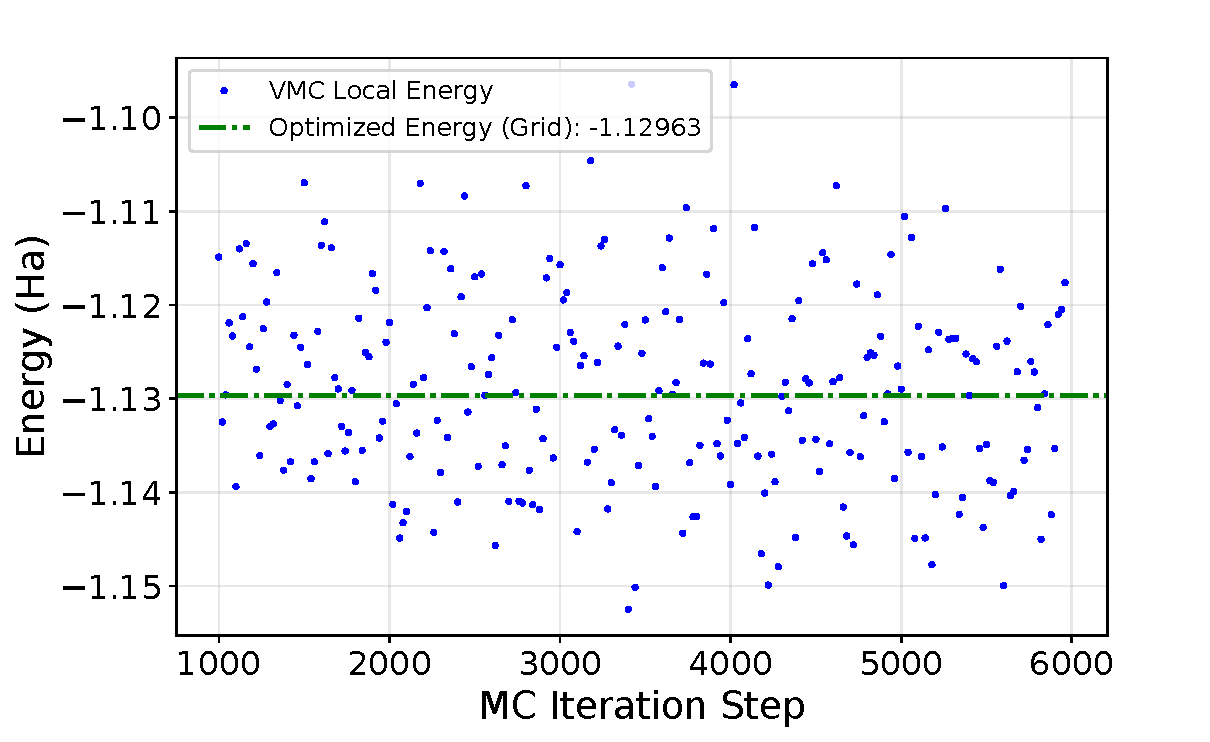
\includegraphics[width=\linewidth]{figs/kegelapan/Energy-Iteration-VMC.pdf}
            {\footnotesize \centering MC sampling at $\alpha = 1.175$}
            
        \column{0.48\textwidth}
            \vspace{1em}
            \centering
            \includegraphics[width=\linewidth]{figs/kegelapan/Energy-Alpha-VMC.pdf}
            {\footnotesize \centering Optimizing the variatonal parameter}
    \end{columns}
\end{frame}

%===========================================================
\begin{frame}{Computational Cost}
%===========================================================
    \begin{enumerate}
        \item \textbf{Wavefunction ($\Psi_T$):} Single update costs
        
        \item \textbf{Sampling Loop:} Updates all $N$ electrons per sweep $$N \times O(N^2) = \mathcal{O}(N^3)$$
        
        \item \textbf{Optimization:} Multiplies cost by steps ($K$) and samples ($M$).
    \end{enumerate}

    \vspace{0.5cm}

    \begin{block}{Final Time Complexity}
        $$T_{VMC} \propto K \times M \times O(N^3)$$
    \end{block}
  
\end{frame}

%===========================================================
\begin{frame}{Why Quantum?}
%===========================================================
    \textbf{The Limit of Classical VMC}  \quad {\small \textcolor{gray}{\textit{\textcolor{co}{When "Good Enough" is not Enough}}}}
    
    \centering
    \includegraphics[width = 0.9\linewidth, height=0.6\paperheight]{figs/kegelapan/meme_VQE.png}
\end{frame}

%===========================================================
\section{Quantum Computing Approach}
%===========================================================

%===========================================================
\begin{frame}{Qubit \& Superposition}
%===========================================================
    % PENTING: Gunakan [c] agar konten di kedua kolom rata tengah vertikal
    \begin{columns}[c]
        
        % --- Kolom Teks ---
        \column{0.6\textwidth}
        \textbf{Classical Bit vs Quantum Bit:}
        \begin{itemize}
            \item Classical: State is either $0$ OR $1$.
            \item Quantum: State can be a linear combination:
            $$ |\psi\rangle = \alpha|0\rangle + \beta|1\rangle $$
            \vspace{-0.5em} % Sedikit mengurangi jarak antar baris
            {\small where $|\alpha|^2 + |\beta|^2 = 1$.}
        \end{itemize}
        
        % --- Kolom Gambar ---
        \column{0.4\textwidth}
        \centering
            \includegraphics[width=0.9\linewidth]{figs/kegelapan/Bloch_Sphere.jpeg}
            \footnotesize{Qubit Representation in Bloch Sphere}
    \end{columns}
\end{frame}

%===========================================================
\begin{frame}{Observables \& Pauli Operators}
%===========================================================
    \textbf{The Language of Qubits:}
    To calculate energy, we must translate the Molecular Hamiltonian ($\hat{H}$) into Qubit Operators.
    
    \vspace{0.5em}
    \textbf{The Pauli Matrices (The Alphabet):}
    \vspace{0.5em}
    \begin{columns}
        \column{0.33\textwidth}
        \centering
        $X = \begin{pmatrix} 0 & 1 \\ 1 & 0 \end{pmatrix}$ 
        
        \column{0.33\textwidth}
        \centering
        $Y = \begin{pmatrix} 0 & -i \\ i & 0 \end{pmatrix}$ 
        
        \column{0.33\textwidth}
        \centering
        $Z = \begin{pmatrix} 1 & 0 \\ 0 & -1 \end{pmatrix}$
    \end{columns}

    \vspace{0.5em}
    \begin{block}{Hamiltonian Mapping}
        The Hamiltonian becomes a weighted sum of Pauli strings:
        $$ \hat{H}_{mol} \longrightarrow \sum_i c_i (P_i \otimes P_j \otimes ...) $$
    \end{block}
\end{frame}

%===========================================================
\begin{frame}{Measurement \& Expectation Value}
%===========================================================

    
    \begin{itemize}
        \item \textbf{Expectation Value ($\langle H \rangle$):} The average outcome of many measurements.
        $$ \langle H \rangle = \langle \psi(\theta) | \hat{H} | \psi(\theta) \rangle $$
    \end{itemize}
    
    \begin{block}{The Process (Shots)}
    \begin{enumerate}
        \item Prepare the state $|\psi(\theta)\rangle$.
        \item Measure the qubits (Collapse to 0 or 1).
        \item Repeat $N$ times (e.g., 1024 shots).
        \item Calculate the statistical average.
    \end{enumerate}
    \end{block}
\end{frame}

%===========================================================
\section{Variational Quantum Algorithm}
%===========================================================

%===========================================================
\begin{frame}{Hamiltonian Mapping}
%===========================================================
  \footnotesize 

    \begin{block}{Stage A: First Quantization}
        \textbf{Process:} Calculate electronic integrals ($h_{pq}, h_{pqrs}$) on CPU.
    \end{block}

    \begin{block}{Stage B: Second Quantization (Fermions)}
        \textbf{Model:} Hamiltonian with operators $a^\dagger$ (create) \& $a$ (annihilate).
         $\hat{H} = \sum h_{pq} a_p^\dagger a_q + \dots$
    \end{block}

    \begin{block}{Stage C: Jordan-Wigner Transform (The Bridge)}
        \textbf{Mapping:} Translate Fermions to Qubits ($a^\dagger \to X, Y, Z$).\\
        \textbf{Mechanism:} Uses Parity Strings to mimic anti-symmetry.
    \end{block}

    \begin{block}{What we want: Qubit Hamiltonian}
        \textbf{Target:} Weighted sum of Pauli Strings to be measured.
         $\hat{H}_{qubit} = \sum c_i (P_0 \otimes P_1 \dots)$
    \end{block}
\end{frame}

%===========================================================
\begin{frame}{Components of VQE}
%===========================================================
    \begin{itemize}
        \setlength\itemsep{0.5em} % Memberi jarak antar poin
        
        \item \textbf{The Objective (Hamiltonian)} \\
        The Qubit Hamiltonian derived from the mapping, represented as a sum of Pauli Strings: 
        % $$ \hat{H}_{qubit} = \sum c_i P_i $$

        \item \textbf{The Ansatz (Quantum Circuit)} \\
        A parameterized circuit $U(\vec{\theta})$ that prepares the trial wavefunction. It utilizes \textit{Superposition} (Rotations) and \textit{Entanglement} (CNOTs).

        \item \textbf{The Estimator (QPU)} \\
        Measures the expectation value via statistical sampling (shots):

        \item \textbf{The Optimizer (Classical CPU)} \\
        Updates the parameters $\vec{\theta}$ using classical methods (e.g., Gradient Descent, SPSA) to minimize $\langle E \rangle$.
    \end{itemize}
\end{frame}

%===========================================================
\begin{frame}{Variational Quantum Eigensolver (VQE)}
%===========================================================
    VQE is a \textcolor{cb}{hybrid algorithm (Quantum + Classical)} designed to find the ground state energy ($E_0$) (e.g. of a molecule) using \textcolor{cr}{Variational Principle}

    \begin{block}{Input}
        \textbf{Hamiltonian ($\hat{H}_{qubit}$):} Decomposed into Pauli Strings $\sum c_i P_i$.\\
        \textbf{Parameters ($\vec{\theta}$):} Rotation angles controlling the Ansatz.
    \end{block}

    \begin{block}{Loop}
        \textbf{QPU (Measure):} Run circuit $U(\vec{\theta})$ and sample expectation values.\\
        \textbf{CPU (Optimize):} Aggregate Energy ($E_{tot}$) and update $\vec{\theta}$ to minimize cost.\\
        \textbf{Repeat:} Iterate until convergence to Ground State.
    \end{block}
\end{frame}

%===========================================================
\begin{frame}{}
%===========================================================
    \begin{tikzpicture}[remember picture, overlay]
        \node[at=(current page.center)] {
            \includegraphics[width=\paperwidth, height=\paperheight]{figs/kegelapan/Circuit VQE.png}
        };
    \end{tikzpicture}
\end{frame}

%===========================================================
\begin{frame}{``Path'' to optimized energy for $\text{H}_2$}
%===========================================================

\begin{center}
            \includegraphics[width=0.6\linewidth]{figs/kegelapan/Energy-Optimization-VQE.pdf}
\end{center}

\end{frame}

%===========================================================
\begin{frame}{Clash of Algorithms: VMC vs. VQE}
%===========================================================
    \begin{table}[]
        \centering
        \renewcommand{\arraystretch}{1.5} % Memberi jarak antar baris agar elegan
        \setlength{\tabcolsep}{8pt} % Memberi jarak antar kolom
        \resizebox{\textwidth}{!}{%
        \begin{tabular}{|l|l|l|}
        \hline
        \rowcolor{black!90} \textbf{Feature} & \textbf{Classical VMC (``The Specialist'')} & \textbf{Quantum VQE (``The Generalist'')} \\ \hline
        
        \textbf{Ansatz Approach} & \textbf{Heuristic Guessing} & \textbf{Scalable Approximation} \\ 
        & (Based on Physical Intuition) & (Systematic Circuit Expansion) \\ \hline
        
        \textbf{Computational Cost} & \textcolor{cb}{${O(N^3)}$} (Polynomial) & \textcolor{cr}{$\mathcal{O}(N)$} (Hamiltonian Terms)* \\ \hline
        
        \textbf{Bottleneck} & \textbf{Sampling Loop} & \textbf{Measurement Loop} \\
        & (Moving Electrons via CPU) & (Shot Noise via QPU) \\ \hline
        
        \textbf{Limit} & Fixed-Node Approximation & Hardware Noise (NISQ) \\ \hline
        \end{tabular}%
        }
    \end{table}
    
    \vspace{0.2cm}
    \tiny{\textit{*Note: VQE scaling can be improved with advanced measurement grouping techniques.}}
\end{frame}
%----------------------------------------------------------- 
\end{document}
%----------------------------------------------------------- 
